\documentclass[10pt,twocolumn]{article}
\usepackage[margin=0.72in]{geometry}
\usepackage{times}
\usepackage{amsmath,amssymb}
\usepackage{booktabs}
\usepackage{graphicx}
\usepackage{url}
\usepackage[hidelinks]{hyperref}
\usepackage{caption}
\captionsetup{font=small}
\setlength{\parskip}{0pt}

\title{\vspace{-1.6em}\Large Who Faces the Capital Constraint?\\
\normalsize\vspace{0.4em}Debt-service burden as a screen for multilateral financing need,
applied to allied defence and to Indo-Pacific grid infrastructure\vspace{-0.4em}}
\author{\normalsize Swastik Sengupta\vspace{-1em}}
\date{}

\begin{document}
\maketitle
\vspace{-3em}

\begin{abstract}
\noindent
Two multilateral financing institutions are being designed at once. The proposed
Defence, Security and Resilience Bank would pool allied credit to fund NATO's
five percent commitment. The Green Grids Initiative, launched by the Prime
Ministers of India and the United Kingdom, exists to move capital into
interregional transmission. Both rest on the same unstated premise: that the
states which most need to build are the ones that can least afford to borrow. I
test that premise with one observed statistic, interest payments as a share of
government revenue, across NATO and the Indo-Pacific. Inside NATO the premise
holds and the numbers are modest. Germany spends $2.48$ percent of revenue on
interest, twenty-one of thirty members exceed it, and the aggregate shortfall
against five percent of GDP is \$1{,}345 billion against only \$54 billion under
the two percent target it replaced. Outside NATO the same measure produces a
dispersion far wider than anything the defence debate contemplates. Across
eighteen Indo-Pacific states the burden runs from $0.47$ percent in Singapore to
$79.9$ percent in Sri Lanka, a range of roughly one hundred and seventy to one.
India, co-founder of the Green Grids Initiative, spends $34.0$ percent of revenue
on interest against the United Kingdom's $8.3$ percent, four times its partner.
Electricity access is near universal across most of the panel, so what binds is
not connection but capital. Every input is observed. Nothing is assumed and
nothing is simulated.
\end{abstract}

\section{Why I started here}

The Defence, Security and Resilience Bank makes a claim anyone can check. Its
public case states that around seventy percent of NATO members face higher
borrowing costs than AAA-rated countries such as Germany \cite{dsrb}. Claims that
specific are unusual in institutional proposals, and I could not find anyone who
had tested it, so I did.

It held, and more exactly than I expected. What kept my attention was something
else. Once the measure was built, running it outside NATO took an afternoon, and
the numbers there are far larger than anything the defence discussion is arguing
about. That comparison is why this paper covers two regions instead of one.

\paragraph{What I claim.} Interest payments as a share of government revenue works
as a screen for which states face a binding \emph{capital} constraint rather than
a \emph{project} constraint. Those need different instruments, and the distinction
is currently drawn rhetorically rather than measured, in both the defence and the
infrastructure debates.

\section{Data}

Everything comes from the World Bank Open Data API, retrieved 27 July 2026, series
last updated 13 July 2026 \cite{worldbank}. I use GDP in current dollars
(\texttt{NY.GDP.MKTP.CD}), military expenditure as a share of GDP
(\texttt{MS.MIL.XPND.GD.ZS}, sourced from SIPRI \cite{sipri}), interest payments
as a share of revenue (\texttt{GC.XPN.INTP.RV.ZS}), access to electricity
(\texttt{EG.ELC.ACCS.ZS}), and population. For each state I take the most recent
non-null observation.

NATO coverage is 32 of 32 on GDP, 31 of 32 on military expenditure, and 31 of 32
on interest payments, leaving 30 members with the complete triple. For the
Indo-Pacific panel of 22 states, interest payments resolve for 18.

\paragraph{On the measure.} Interest over revenue is a realised fiscal outcome,
not a market price. It embeds the existing debt stock and its maturity profile
alongside the current cost of new issuance, so it measures debt-service burden
rather than marginal borrowing cost. The two can diverge. I return to this in
Section~\ref{sec:limits}, because it matters most for the single largest result.

\section{NATO: the claim holds, the target moved}

\begin{figure}[t]
\centering
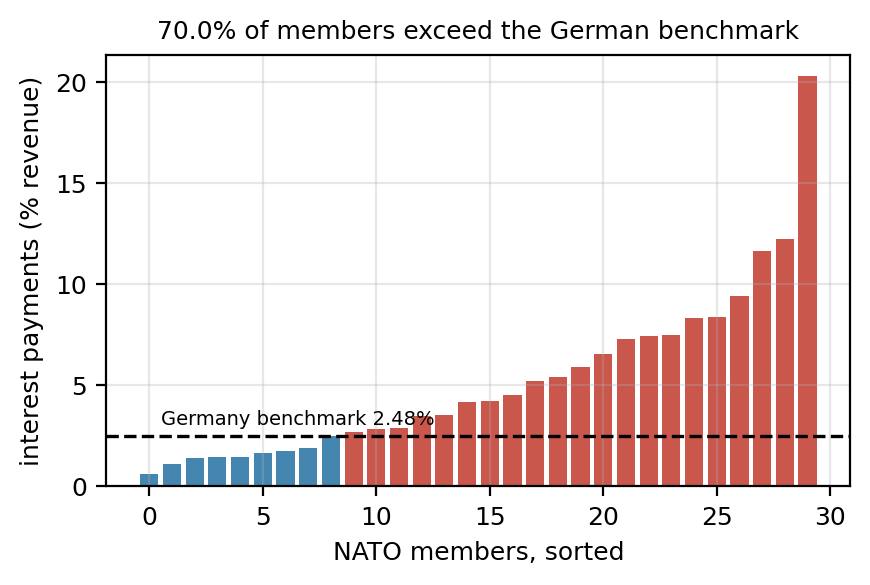
\includegraphics[width=0.94\columnwidth]{figures/fig3_verification.png}
\caption{NATO members sorted by interest burden. The dashed line is Germany.
Twenty-one of thirty lie above it.}
\label{fig:verify}
\end{figure}

Germany's interest payments take $2.48$ percent of government revenue. Twenty-one
of thirty members with complete data are above it, which is $70.0$ percent
(Figure~\ref{fig:verify}). The Bank says around seventy. Agreement that close on a
proxy the Bank does not itself cite is closer than the construction deserves, and
I read it as confirming direction and magnitude rather than the decimal. The claim
is sound.

The more useful number is what the commitment costs. Against two percent of GDP
the alliance is nearly compliant and the aggregate shortfall is \$54 billion.
Against five percent it is \$1{,}345 billion, and no member currently meets it.
The financing problem is not inherited from chronic underspending. It was created
by raising the benchmark, which means the demand arrived recently and arrived
everywhere at once.

It is also concentrated. Taking the NATO median burden of $4.21$ percent as the
threshold, fifteen members carry both an above-median burden and a shortfall, and
those fifteen hold $78.6$ percent of the total.

\section{The result I did not expect}

\begin{figure}[t]
\centering
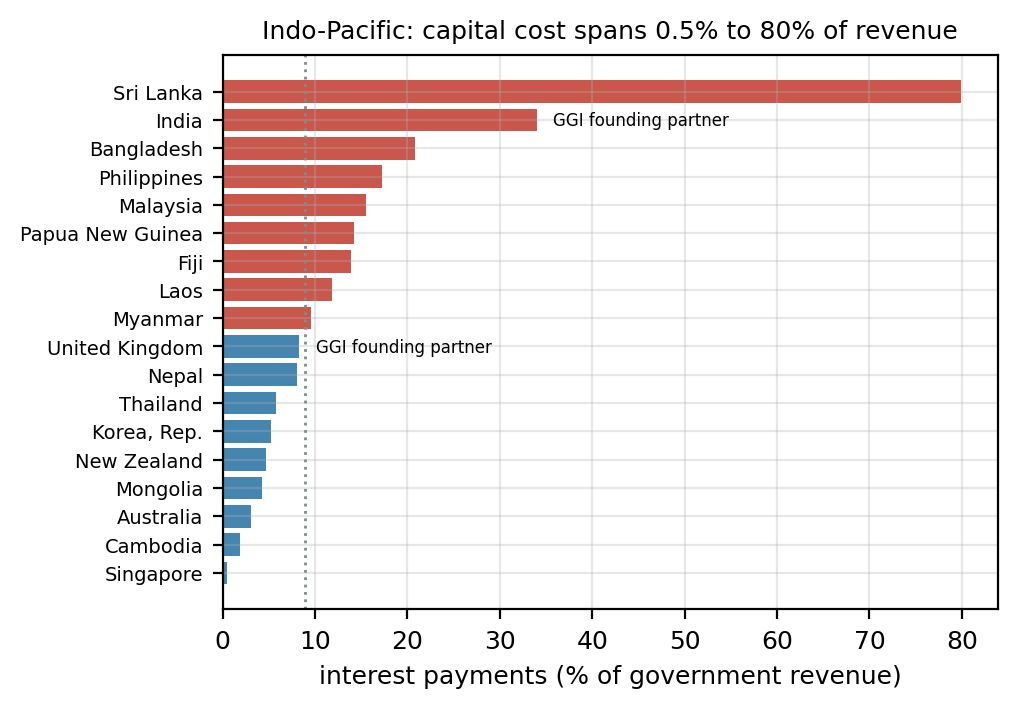
\includegraphics[width=0.94\columnwidth]{figures/fig4_indopacific.png}
\caption{Indo-Pacific and GGI-relevant states by interest burden. The dotted line
is the panel median at $8.94$ percent.}
\label{fig:ip}
\end{figure}

\begin{table}[t]
\centering\small
\caption{Interest payments as a share of government revenue, selected Indo-Pacific
states, most recent observation.}
\label{tab:ip}
\begin{tabular}{lrr}
\toprule
state & int.\ \% revenue & electricity access \% \\
\midrule
Sri Lanka        & 79.87 & 100.0 \\
India            & 33.98 & 99.9 \\
Bangladesh       & 20.83 & 99.5 \\
Philippines      & 17.29 & 94.8 \\
Malaysia         & 15.55 & 100.0 \\
Papua New Guinea & 14.18 & 43.3 \\
Fiji             & 13.86 & 95.9 \\
Laos             & 11.85 & 96.5 \\
Myanmar          & 9.56  & 80.4 \\
United Kingdom   & 8.32  & 100.0 \\
Nepal            & 8.02  & 97.9 \\
Thailand         & 5.76  & 100.0 \\
Australia        & 3.08  & 100.0 \\
Singapore        & 0.47  & 100.0 \\
\bottomrule
\end{tabular}
\end{table}

The defence debate treats a spread from $2.5$ to $20$ percent of revenue as
serious enough to justify building a new multilateral bank. The identical measure
across the Indo-Pacific returns a spread from $0.47$ percent in Singapore to
$79.9$ percent in Sri Lanka (Table~\ref{tab:ip}, Figure~\ref{fig:ip}). That is
roughly one hundred and seventy to one, against NATO's eight to one.

Sri Lanka is an extreme case reflecting sovereign default and restructuring rather
than ordinary conditions, and should not be read as a steady state. The
distribution is wide without it.

\paragraph{The comparison that matters most.} The Green Grids Initiative was
launched by the Prime Ministers of India and the United Kingdom \cite{ggi}. India
spends $34.0$ percent of government revenue on interest. The United Kingdom spends
$8.3$ percent. Two states co-founding one multilateral platform face capital costs
differing by a factor of four. Any instrument designed to mobilise capital across
that partnership has to work at both ends of it.

\paragraph{Access is not the binding constraint.} Electricity access is at or near
universal across most of the panel: India $99.9$ percent, Sri Lanka and Malaysia
$100$, Bangladesh $99.5$. What these states need is not connection but transmission
and interregional capacity, which is the Green Grids brief. So for most of them the
question is not whether the physical requirement exists. It is whether capital can
be raised against it at a price that makes projects bankable.

Papua New Guinea is the exception and deserves separating. It carries both a high
burden at $14.2$ percent and electricity access of only $43.3$ percent, so both
constraints bind at once. It needs a different instrument from India, which has
the connections and the pipeline but pays four times what the United Kingdom pays
to borrow.

\section{What the screen is for}

Both institutions face the same design question: who is the customer. This answers
a narrow version of it. A state above the panel median on debt-service burden
faces a capital constraint, and concessional or pooled financing changes what it
can build. A state below the median does not, and for it the binding constraint is
pipeline, permitting, or offtake, none of which a lending facility fixes.

That distinction is currently asserted rather than measured in both debates. It
takes one public indicator and an afternoon to measure.

\section{Limitations}
\label{sec:limits}

The measure is realised burden, not marginal cost. A state with cheap new issuance
but a large legacy stock scores as constrained. The clearest case is the United
States, which on this screen carries the highest burden in NATO at $20.3$ percent
of revenue while also holding the largest absolute shortfall at \$486 billion,
$36$ percent of the alliance total. On the Bank's own criterion it is the single
largest potential borrower, which sits awkwardly with a pooled-rating rationale
built to extend larger members' credit to smaller ones. It may equally reflect what
the proxy cannot see, since reserve-currency issuance and a very large legacy stock
pull in opposite directions. I flag it rather than resolve it.

The gap calculation is a static identity at current GDP, not a forecast, and it
assumes the five percent target binds. Panels are not perfectly contemporaneous:
military expenditure is 2024 while interest payments are 2023 or 2024. Central
government debt resolves for only eight NATO members and is excluded. Four
Indo-Pacific states drop for missing interest data.

Nothing here evaluates whether either institution would work. I have measured a
constraint and identified who it binds. Whether pooled multilateral lending is the
right response is a separate question.

\section{Conclusion}

One public indicator, retrieved in an afternoon, verifies the Defence, Security and
Resilience Bank's headline claim to the decimal, and then shows that the
capital-cost dispersion the Bank was designed around is an order of magnitude
smaller in NATO than in the Indo-Pacific. The two states that founded the Green
Grids Initiative differ from each other by a factor of four on the same measure.
Across most of that region electricity access is already near universal, so what
binds is capital rather than connection.

If a screen this cheap separates states that need concessional capital from states
that need a project pipeline, it is worth running before the instruments are
designed rather than after.

\begin{thebibliography}{9}\small
\bibitem{dsrb} Defence, Security and Resilience Bank Development Group, ``What is
the DSRB,'' \url{https://www.dsrb.org/what-is-the-dsrb}, retrieved 27 July 2026.
\bibitem{atlanticcouncil} R. Murray, ``How a new global defense bank can solve US
and allied funding problems,'' Atlantic Council in-depth research report.
\bibitem{worldbank} World Bank, World Development Indicators, Open Data API,
\url{https://api.worldbank.org/v2}, series last updated 13 July 2026.
\bibitem{sipri} Stockholm International Peace Research Institute, Military
Expenditure Database, distributed as World Bank series
\texttt{MS.MIL.XPND.GD.ZS}.
\bibitem{ggi} Green Grids Initiative, launched by the Prime Ministers of India and
the United Kingdom under One Sun One World One Grid.
\bibitem{skipper2026} G. Skipper, ``Follow the money: finance and the future of
allied economic statecraft,'' War on the Rocks, March 2026.
\bibitem{murrayfrolund} F. Murray and L. Fr\o lund, ``From sovereign yards to
shared gardens: securing technological advantage through collective economic
security,'' MIT Murray Lab.
\bibitem{nato} North Atlantic Treaty Organization, Defence Expenditure of NATO
Countries, annual series.
\end{thebibliography}

\end{document}
